% Elemento de volume em coordenadas cartesianas
% Feito para o ÉguaTeX (eguatex.com.br). Uso livre (CC0 1.0).
%
% Compile e pronto: sai só a figura, em PDF.
% Para pôr no seu trabalho, use o PDF com \includegraphics ou copie
% o bloco tikzpicture para dentro de uma figure.
\documentclass[tikz,border=4pt]{standalone}
\usepackage[T1]{fontenc}
\usepackage{lmodern}
\usetikzlibrary{patterns.meta}

\begin{document}
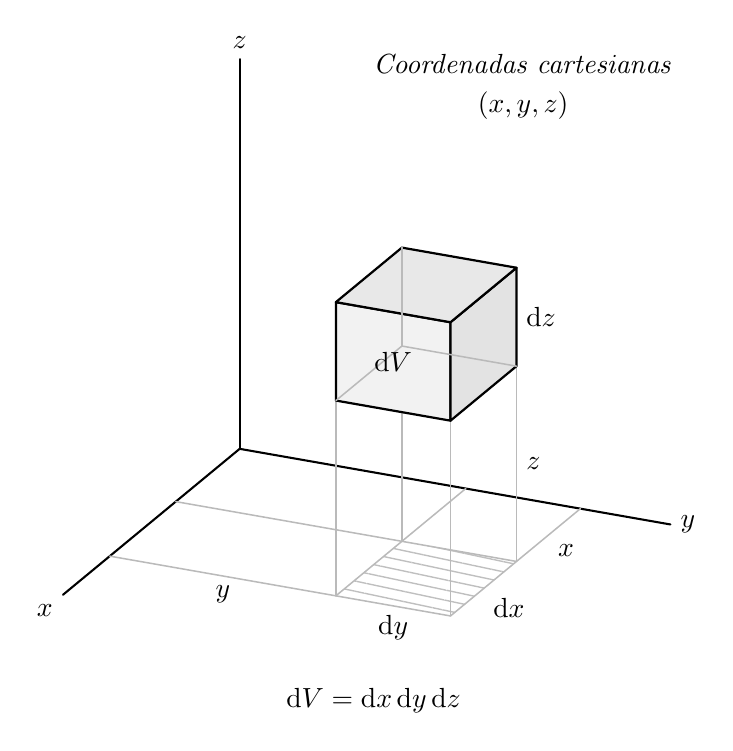
\begin{tikzpicture}[
  x={(-0.4435cm,-0.3663cm)}, y={(0.9768cm,-0.1715cm)}, z={(0cm,1cm)},
  line cap=round, line join=round,
  eixo/.style={line width=0.75pt},
  aresta/.style={line width=0.8pt},
  guia/.style={line width=0.55pt, black!27}]

% Mude estes números e o desenho e os rótulos acompanham.
\def\xa{1.83} \def\xb{3.72}  % x e x + dx
\def\ya{2.94} \def\yb{4.43}  % y e y + dy
\def\za{2.48} \def\zb{3.73}  % z e z + dz

\draw[eixo] (0,0,0) -- (5.06,0,0) node[below left]  {$x$};
\draw[eixo] (0,0,0) -- (0,5.6,0)  node[right]       {$y$};
\draw[eixo] (0,0,0) -- (0,0,4.95) node[above]       {$z$};

\fill[pattern={Lines[angle=-12, distance=3.6pt, line width=0.5pt]}, pattern color=black!25]
  (\xa,\ya,0) -- (\xb,\ya,0) -- (\xb,\yb,0) -- (\xa,\yb,0) -- cycle;
\draw[guia] (\xb,0,0) -- (\xb,\yb,0) -- (0,\yb,0);
\draw[guia] (\xa,0,0) -- (\xa,\yb,0);
\draw[guia] (0,\ya,0) -- (\xb,\ya,0);

\foreach \x/\y in {\xa/\ya, \xb/\ya, \xb/\yb, \xa/\yb}
  \draw[guia] (\x,\y,0) -- (\x,\y,\za);

\filldraw[aresta, fill=black!5]
  (\xb,\ya,\za) -- (\xb,\yb,\za) -- (\xb,\yb,\zb) -- (\xb,\ya,\zb) -- cycle;
\filldraw[aresta, fill=black!11]
  (\xb,\yb,\za) -- (\xa,\yb,\za) -- (\xa,\yb,\zb) -- (\xb,\yb,\zb) -- cycle;
\filldraw[aresta, fill=black!9]
  (\xa,\ya,\zb) -- (\xb,\ya,\zb) -- (\xb,\yb,\zb) -- (\xa,\yb,\zb) -- cycle;
\draw[guia] (\xb,\ya,\za) -- (\xa,\ya,\za) -- (\xa,\yb,\za);
\draw[guia] (\xa,\ya,\za) -- (\xa,\ya,\zb);

\node at ({\xb},{(\ya+\yb)/2},{(\za+\zb)/2}) {$\mathrm{d}V$};
\path (\xa,\yb,\za) -- (\xa,\yb,\zb) node[midway, right] {$\mathrm{d}z$};
\path (\xa,\yb,0)   -- (\xa,\yb,\za) node[midway, right] {$z$};
\path (0,\yb,0)     -- (\xa,\yb,0)   node[midway, below right] {$x$};
\path (\xa,\yb,0)   -- (\xb,\yb,0)   node[midway, below right] {$\mathrm{d}x$};
\path (\xb,0,0)     -- (\xb,\ya,0)   node[midway, below] {$y$};
\path (\xb,\ya,0)   -- (\xb,\yb,0)   node[midway, below] {$\mathrm{d}y$};

\node[align=center] at (3.6cm,4.6cm) {\textit{Coordenadas cartesianas}\\[2pt] $(x,y,z)$};
\node at (1.7cm,-3.2cm) {$\mathrm{d}V=\mathrm{d}x\,\mathrm{d}y\,\mathrm{d}z$};
\end{tikzpicture}
\end{document}
